\documentclass[journal]{IEEEtran}

\usepackage{enumerate}
\usepackage[binary-units=true]{siunitx}
\usepackage{amsfonts,amssymb,amsmath}
\DeclareMathOperator{\Tr}{Tr}

\usepackage{bm,bbm}
\usepackage{subfigure}
\usepackage{array}
\usepackage{breqn}

\DeclareMathOperator*{\argmax}{\arg\!\max}

\usepackage{booktabs}

\usepackage[export]{adjustbox}
\usepackage{multirow}
\usepackage{color}
\usepackage[noabbrev]{cleveref}
\usepackage{cite}

\usepackage{times}
\usepackage{multicol}
\usepackage{graphicx}
\usepackage{underscore}
\graphicspath{{../../Images/PNG/}{../../Images/PDF/}{../../Plots/}}

\begin{document}
	
\title{Road Detection in SAR Images using Simulated Data}
	
\author{Xiangrong Zhang,~\IEEEmembership{Senior Member,~IEEE,}~Zhu Xiao Qian~\IEEEmembership{Student Member,~IEEE,},~and~Alejandro~C.~Frery,~\IEEEmembership{Senior Member,~IEEE}%
	\thanks{X.~Zhang and Z.X. Qian are with the  (e-mail: xrzhang@mail.xidian.edu.cn)}% 
	\thanks{Alejandro~C.~Frery is with the Laborat\'orio de Computa\c c\~ao Cient\'ifica e An\'alise Num\'erica, Universidade Federal de Alagoas, Macei\'o, Brazil, and with the Key Lab of Intelligent Perception and Image Understanding of the Ministry of Education, Xidian University, Xi'an, China.. (e-mail: acfrery@laccan.ufal.br)}% <-this % stops a space
	\thanks{Manuscript received XXX, 2019; revised YYY, 2019.}
	}

\IEEEtitleabstractindextext{%
\begin{abstract}
About NN\dots
We use samples from the Potts model\dots
\end{abstract}

\begin{IEEEkeywords}
SAR, 
speckle, 
simulation, 
\dots
\end{IEEEkeywords}}

\maketitle

\IEEEdisplaynontitleabstractindextext
\IEEEpeerreviewmaketitle

\section{Proof-of-Concept}\label{sec:SamplingMethodology}

We are able to simulate an arbitrary number of samples using a road map.

Consider the model for image formation proposed by Geman and Geman~\cite{geman84}, and later extended by Bustos and Frery~\cite{buseucam92}.
This model states that the observed image $Z$ is the result of a transformation $\tau$ of the unobserved truth $X$.
The transformation consists of:
$phi$, a possibly nonlinear pointwise transformation of the truth;
$H$, a local degradation of $\phi(X)$;
$Y$, the noise in the form of a random field, that enters the model by pointwise operations $\odot$.
With this, we have:
\begin{equation}
Z = H(\phi(X)) \odot Y.
\end{equation}

Our truth is a map of roads, as illustrated in Fig.~\ref{image:Roads}, which we want to retrieve from a SAR image of the scene.
Figs.~\ref{image:SingleLook} and~\ref{image:ThreeLooks} illustrate two simulated observed SAR images of the scene whose truth is the map of roads.

Winkler~\cite{Winkler2006} provides details about the use of the Potts model in image analysis.
We use the Swendsen-Wang algorithm~\cite{SwendsenWang87} for sampling from this model.

\begin{figure*}[hbt]
\centering
\subfigure[Roads\label{image:Roads}]{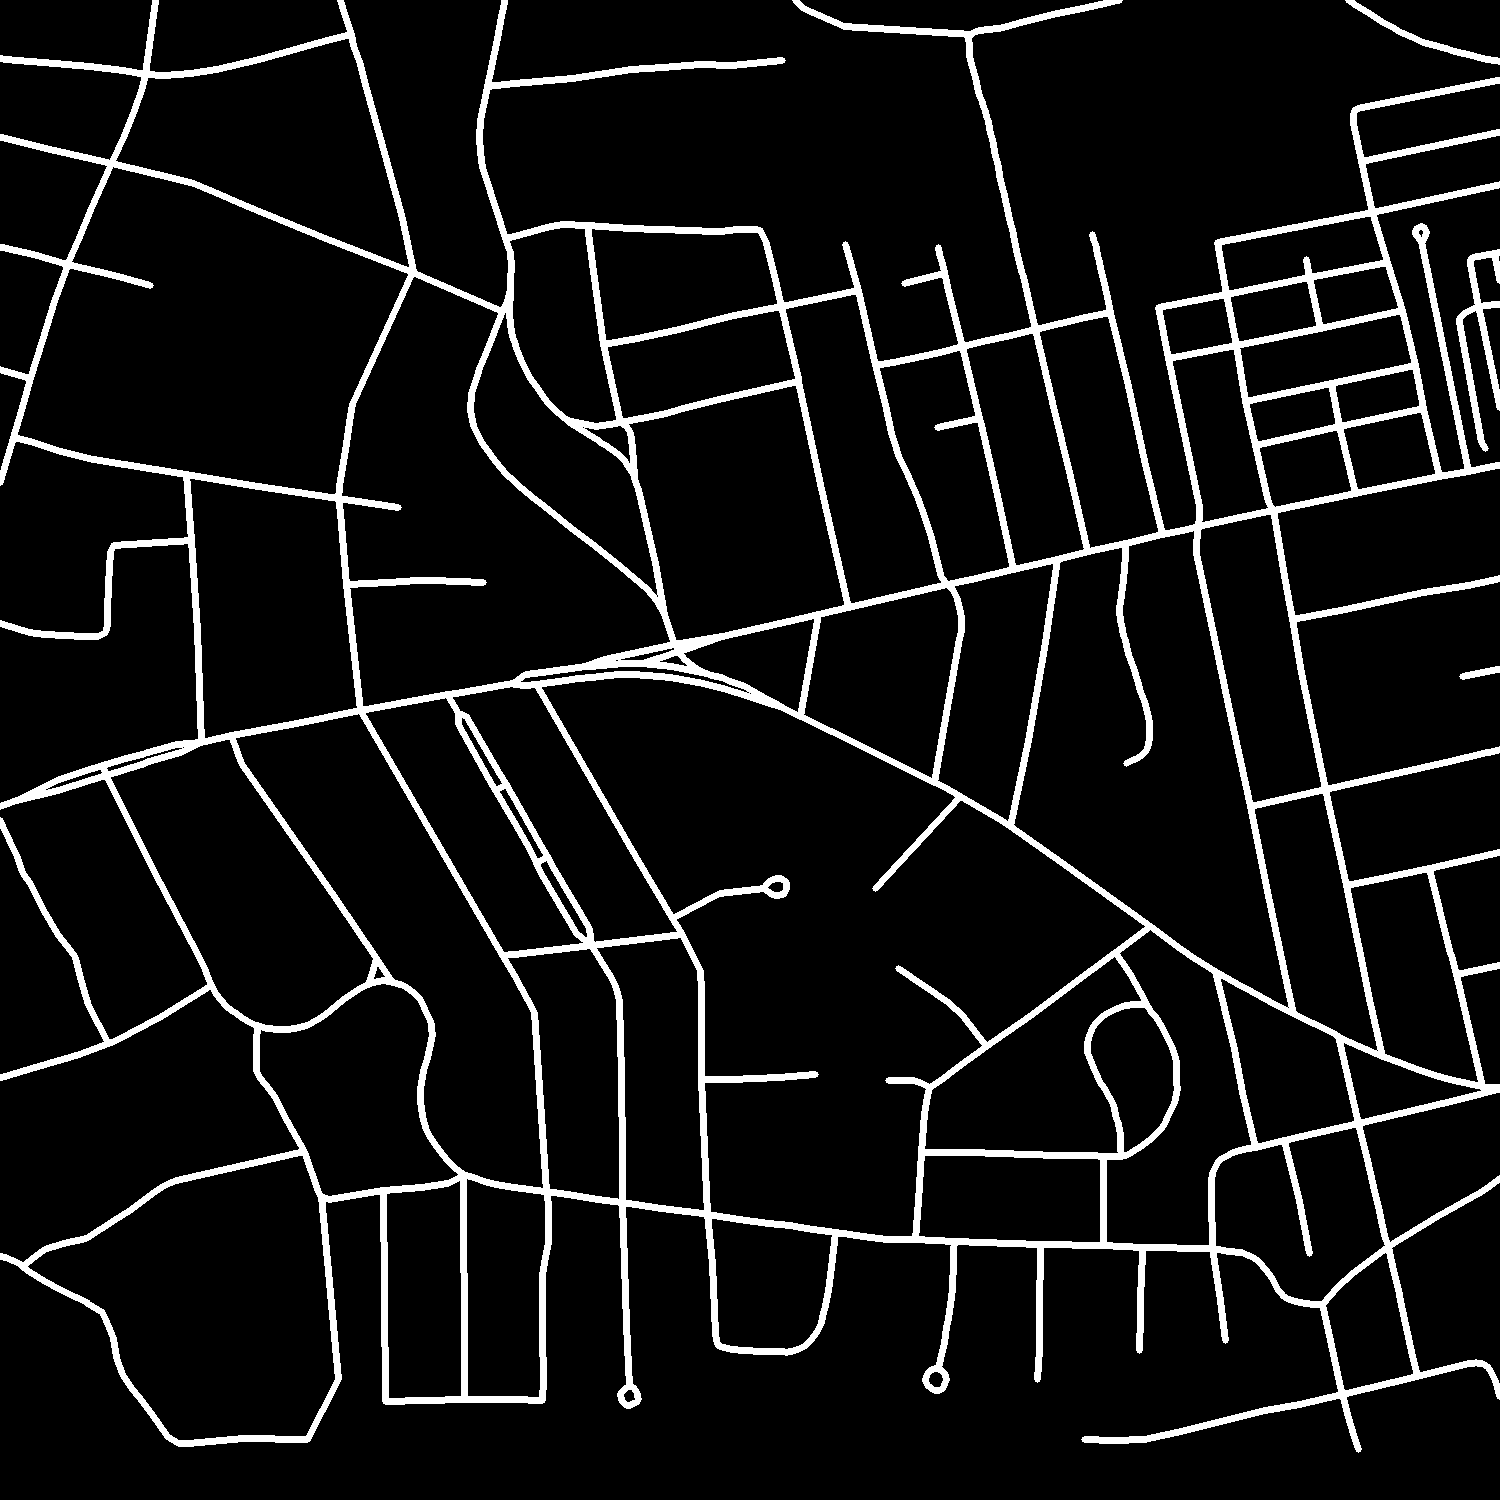
\includegraphics[width=.32\linewidth]{1052873515}}
\subfigure[Simulated SAR image, single look\label{image:SingleLook}]{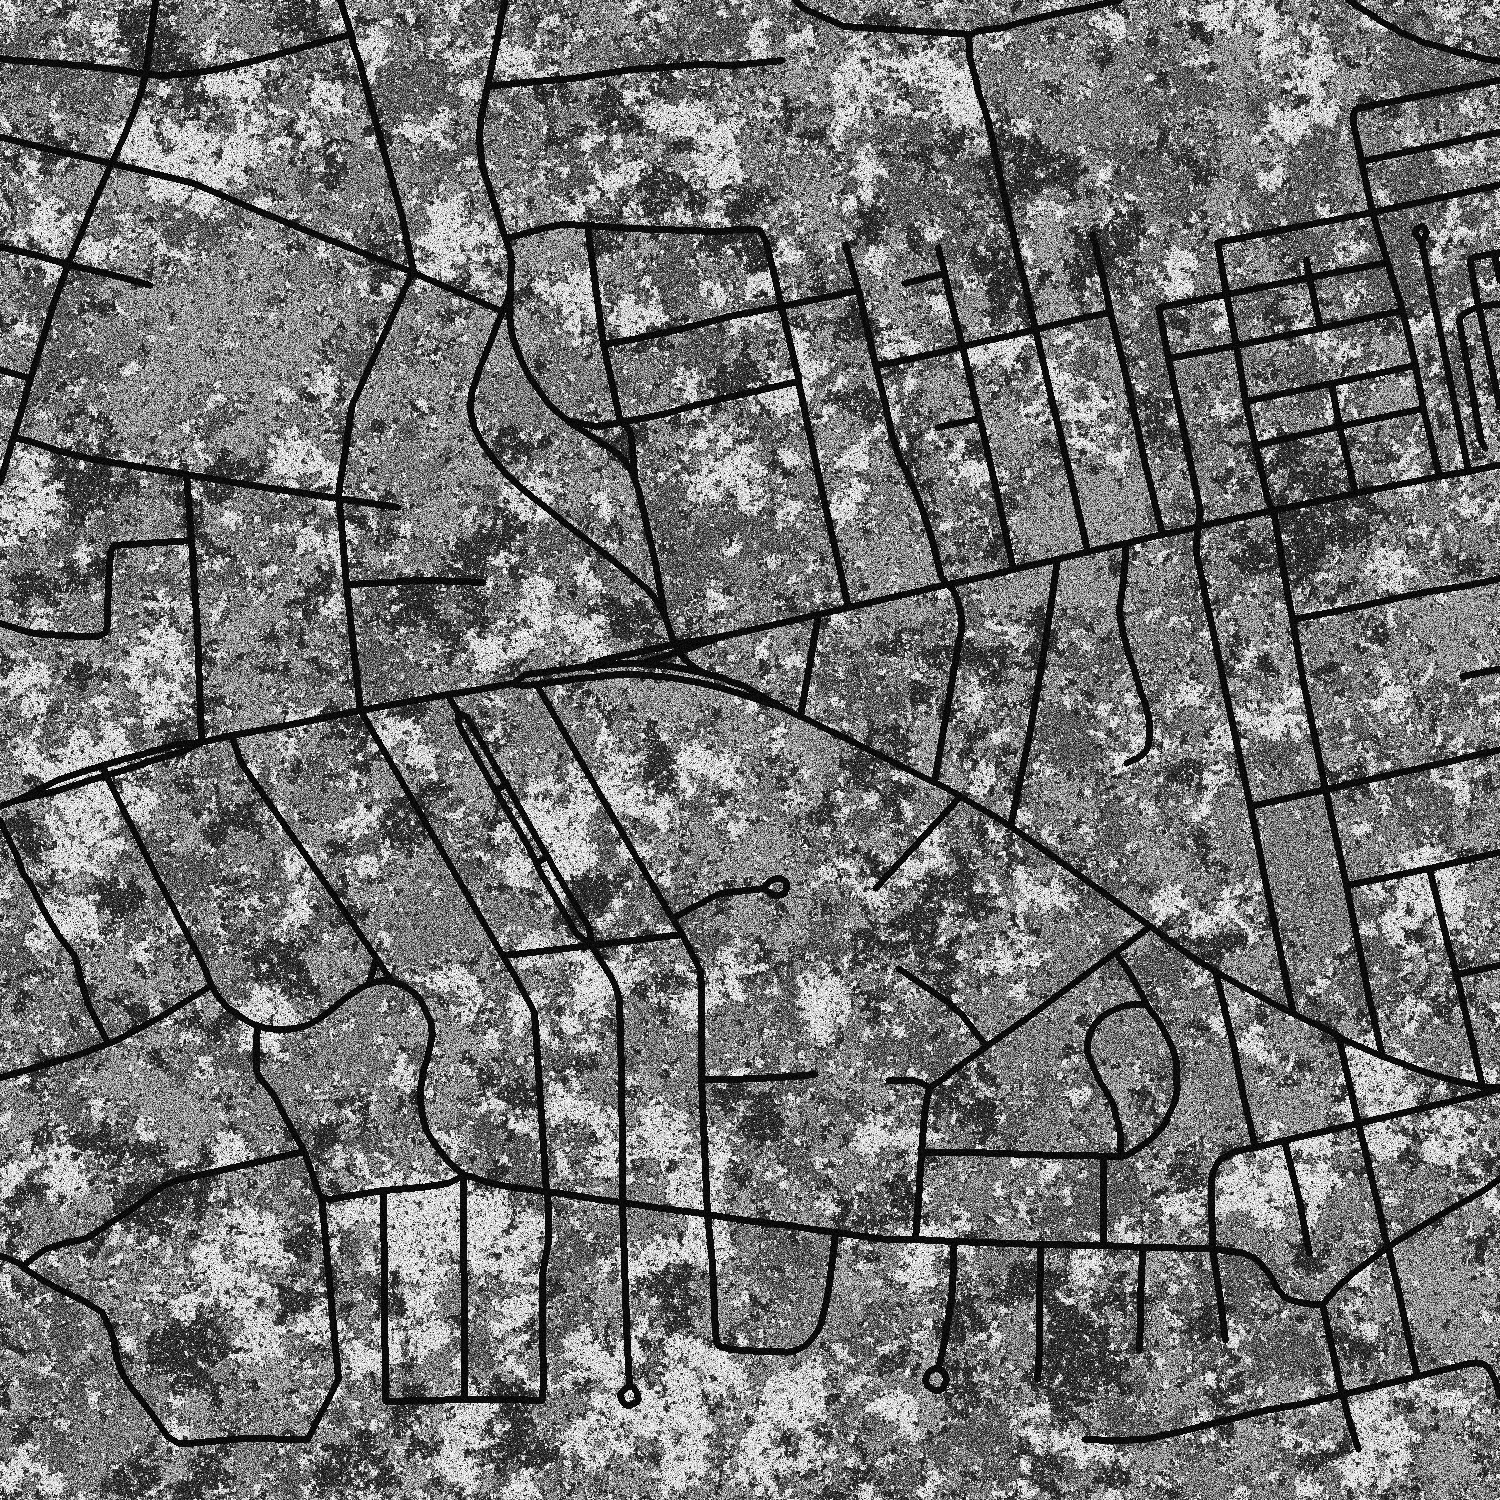
\includegraphics[width=.32\linewidth]{1look}}
\subfigure[Simulated SAR image, three looks\label{image:ThreeLooks}]{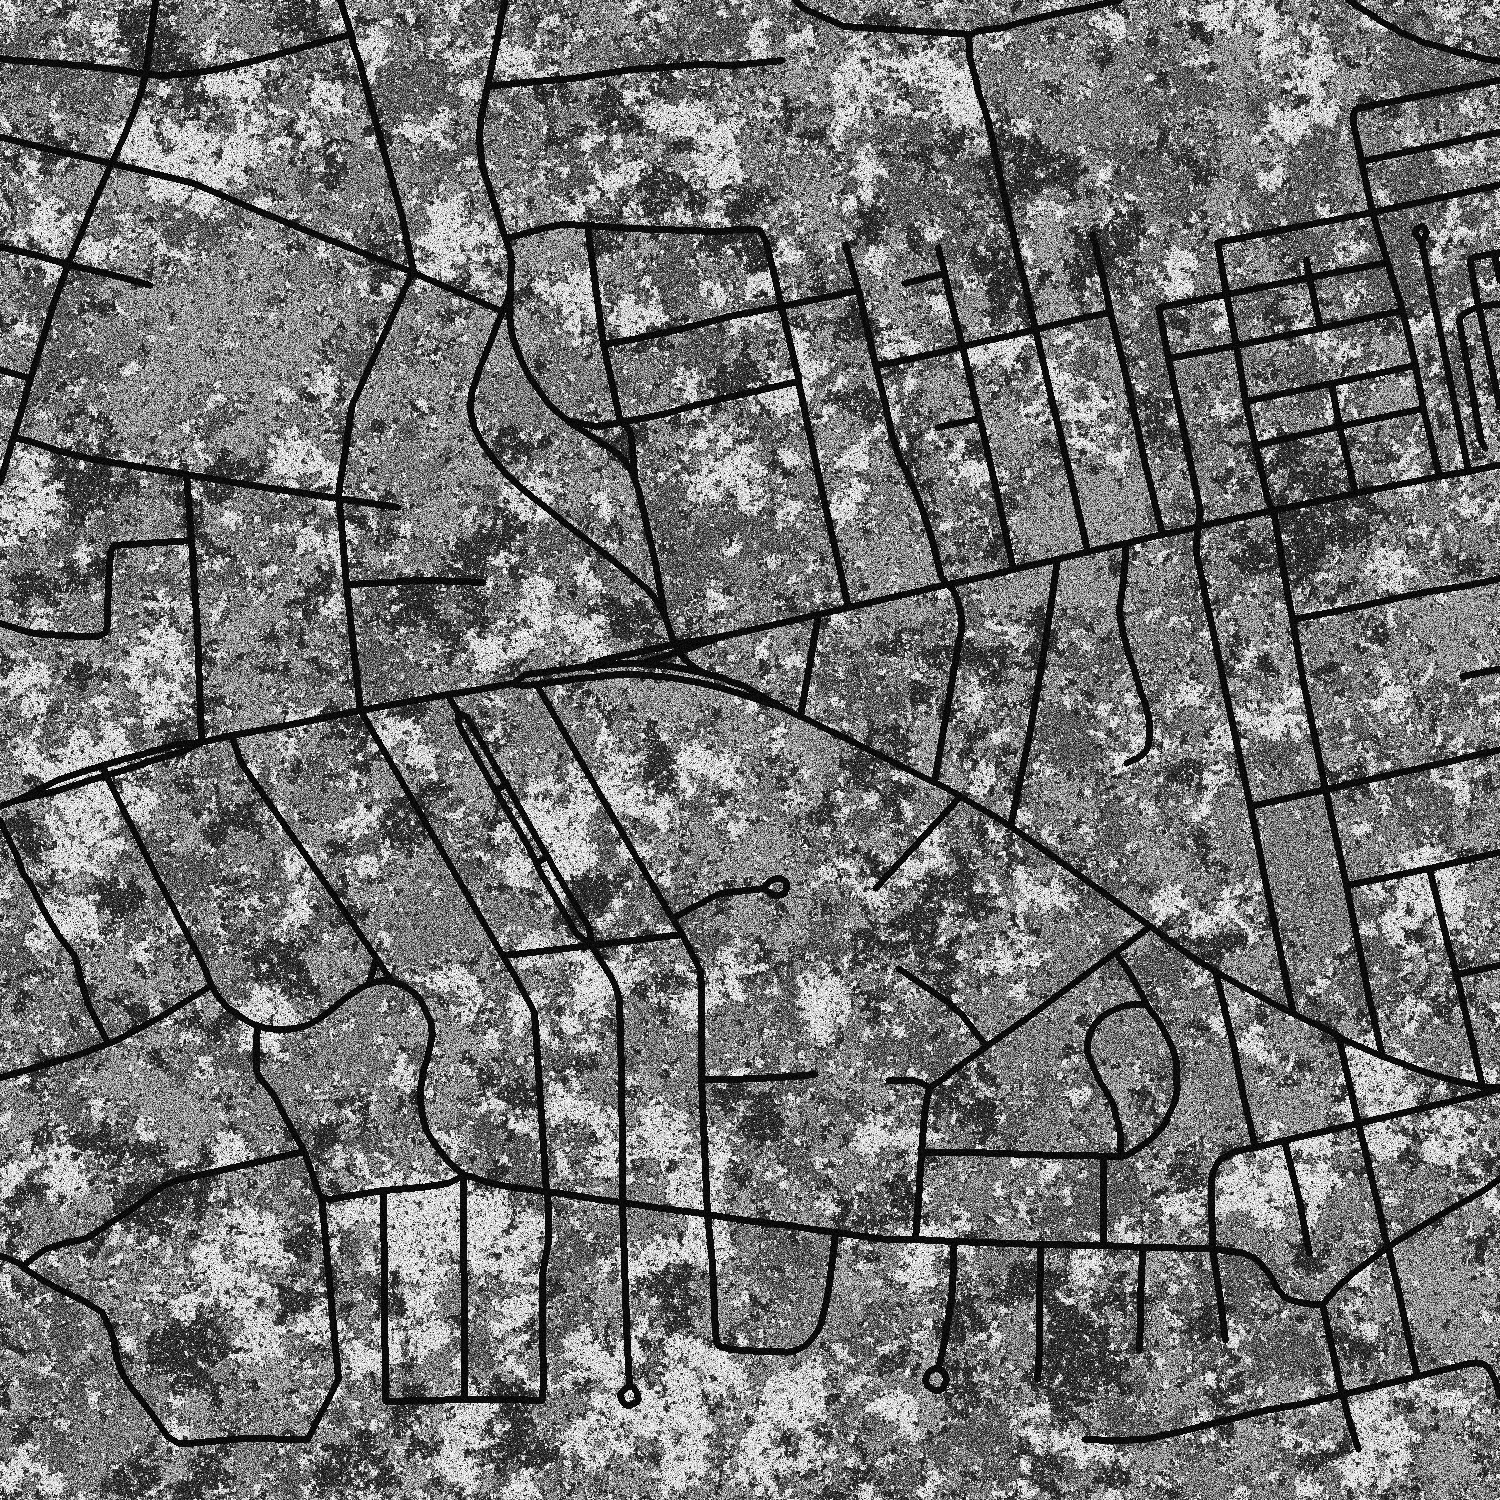
\includegraphics[width=.32\linewidth]{3looks}}
\caption{Example of the proposed pipeline}\label{fig:Pipeline}
\end{figure*}

\bibliographystyle{IEEEtran}
\bibliography{../Common/bibliography}

\end{document}
